\section{Buildroot community: support and contribution}

\begin{frame}{Documentation}
  \begin{itemize}
  \item Buildroot comes with its own documentation
  \item Pre-built versions available at
    \url{http://buildroot.org/docs.html} (PDF, HTML, text)
  \item Source code of the manual located in \code{docs/manual} in the
    Buildroot sources
    \begin{itemize}
    \item Written in {\em Asciidoc} format
    \end{itemize}
  \item The manual can be built with:
    \begin{itemize}
    \item \code{make manual}
    \item or just \code{make manual-html}, \code{make manual-pdf},
      \code{make manual-epub}, \code{make manual-text}, \code{make
        manual-split-html}
    \item A number of tools need to be installed on your machine,
      see the manual itself.
    \end{itemize}
  \end{itemize}
\end{frame}

\begin{frame}{Getting support}
  \begin{itemize}
  \item Free support
    \begin{itemize}
    \item The {\em mailing list} for e-mail discussion\\
      {\footnotesize \url{http://lists.busybox.net/mailman/listinfo/buildroot}}\\
      1300+ subscribers, quite heavy traffic.
    \item The IRC channel, {\tt \#buildroot} on the Freenode network,
      for interactive discussion\\
      100+ people, most available during European daylight hours
    \item Bug tracker\\
      \url{https://bugs.busybox.net/buglist.cgi?product=buildroot}
    \end{itemize}
  \item Commercial support
    \begin{itemize}
    \item A number of embedded Linux services companies, including
      Free Electrons, can provide commercial services around
      Buildroot.
    \end{itemize}
  \end{itemize}
\end{frame}

\begin{frame}{Tips to get free support}
  \begin{itemize}
  \item If you have a build issue to report:
    \begin{itemize}
    \item Make sure to reproduce after a \code{make clean all} cycle
    \item Include the Buildroot version, Buildroot \code{.config} that
      reproduces the issue, and last 100-200 lines of the build
      output in your report.
    \item Use {\em pastebin} sites like \code{http://code.bulix.org}
      when reporting issues over IRC.
    \end{itemize}
  \item The community will be much more likely to help you if you use
    a recent Buildroot version.
  \end{itemize}
\end{frame}

\begin{frame}{Release schedule}
  \begin{itemize}
  \item The Buildroot community publishes stable releases every three
    months.
  \item YYYY.02, YYYY.05, YYYY.08 and YYYY.11 every year.
  \item The three months cycle is split in two periods
    \begin{itemize}
    \item Two first months of active development
    \item One month of stabilization before the release
    \end{itemize}
  \item At the beginning of the stabilization phase, \code{-rc1} is
    released.
  \item Several \code{-rc} versions are published during this
    stabilization phase, until the final release.
  \item Development not completely stopped during the stabilization, a
    \code{next} branch is opened.
  \end{itemize}
\end{frame}

\begin{frame}{Contribution process}
  \begin{itemize}
  \item Contributions are made in the form of patches
  \item Created with \code{git} and sent by e-mail to the mailing list
    \begin{itemize}
    \item Use \code{git send-email} to avoid issues
    \end{itemize}
  \item The patches are reviewed, tested and discussed by the
    community
    \begin{itemize}
    \item You may be requested to modify your patches, and submit
      updated versions
    \end{itemize}
  \item Once ready, they are applied by the project maintainer Peter
    Korsgaard, or the interim maintainer Thomas Petazzoni.
  \item Some contributions may be rejected if they do not fall within
    the Buildroot principles/ideas, as discussed by the community.
  \end{itemize}
\end{frame}

\begin{frame}{Patchwork}
  \begin{itemize}
  \item Tool that records all patches sent on the mailing list
  \item Allows the community to see which patches need review/testing,
    and the maintainers which patches can be applied.
  \item Everyone can create an account to manage his own patches
  \item \url{http://patchwork.buildroot.org/}
  \end{itemize}

  \begin{center}
    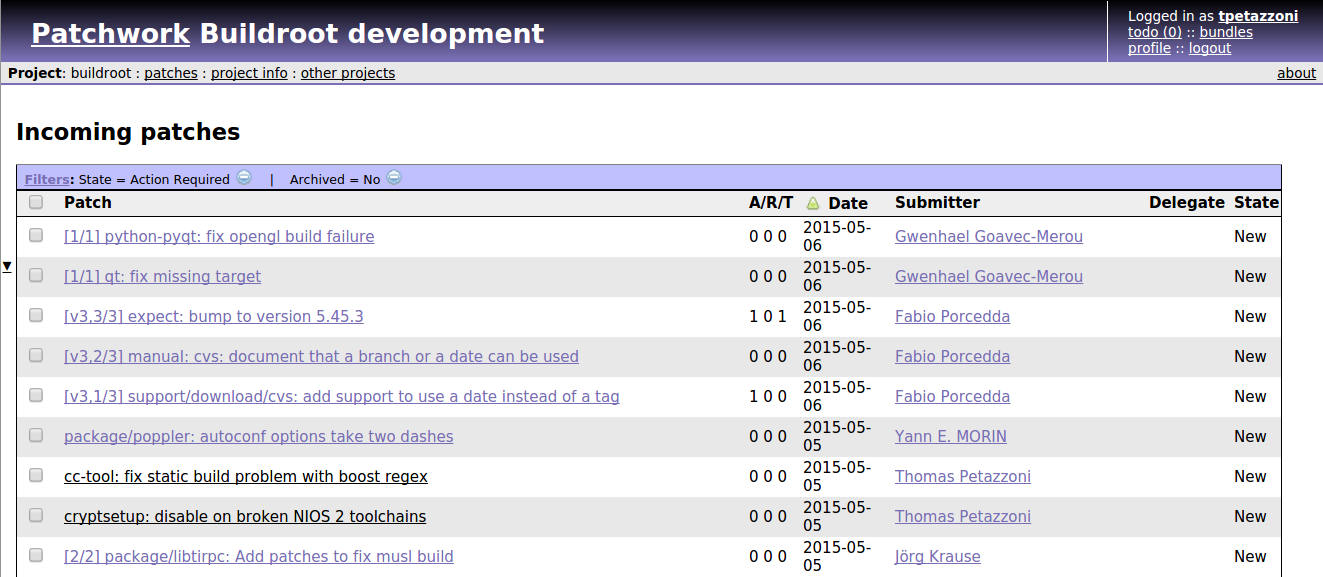
\includegraphics[width=\textwidth]{slides/buildroot-support-contribution/patchwork.png}
  \end{center}
\end{frame}

\begin{frame}{Automated build testing}
  \begin{itemize}
  \item The enormous number of configuration options in Buildroot make
    it very difficult to test all combinations.
  \item Random configurations are therefore built 24/7 by multiple
    machines.
    \begin{itemize}
    \item Random choice of architecture/toolchain combination from a
      pre-defined list
    \item Random selection of packages using \code{make
        randpackageconfig}
    \item Random enabling of features like static library only, or
      \code{BR2_ENABLE_DEBUG=y}
    \end{itemize}
  \item Scripts and tools publicly available at
    \url{http://git.buildroot.net/buildroot-test/}
  \item Results visible at \url{http://autobuild.buildroot.org/}
  \item Daily e-mails with the build results of the past day
  \end{itemize}
\end{frame}

\begin{frame}{autobuild.buildroot.org}
  \begin{center}
    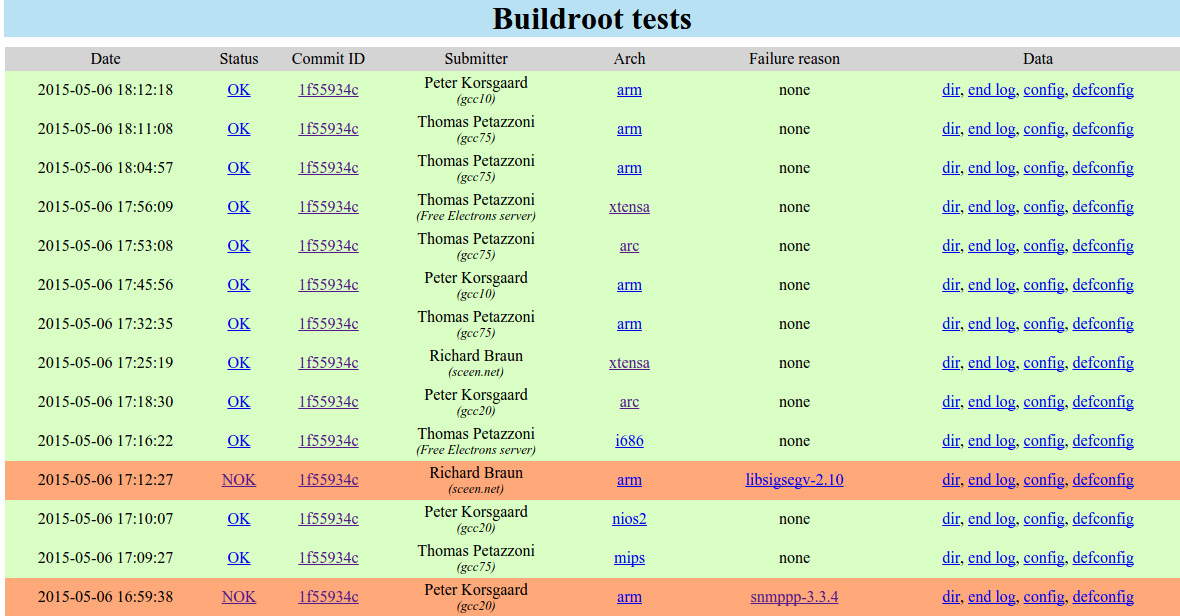
\includegraphics[width=\textwidth]{slides/buildroot-support-contribution/autobuild.png}
  \end{center}
\end{frame}

\begin{frame}[fragile]{Autobuild daily reports}

{\tiny
\begin{verbatim}
From: Thomas Petazzoni <thomas.petazzoni@free-electrons.com>
To: buildroot@uclibc.org
Subject: [Buildroot] [autobuild.buildroot.net] Build results for 2015-05-05
Date: Wed,  6 May 2015 08:30:17 +0200 (CEST)

Build statistics for 2015-05-05
===============================

        success : 301
       failures : 50 
       timeouts : 1  
          TOTAL : 352

Classification of failures by reason
====================================

freerdp-770c67d340d5f0a7b48... | 6 
              postgresql-9.4.1 | 5 
            python-pyqt-4.11.3 | 5 

Detail of failures
===================

     powerpc | boost-1.57.0 | NOK | http://autobuild.buildroot.net/results/b64fd94a8ccff7fa8...
        bfin | cc-tool-0.26 | NOK | http://autobuild.buildroot.net/results/5f84d5696a52c7541...
      xtensa | cc-tool-0.26 | NOK | http://autobuild.buildroot.net/results/d971db839e84480a5...
\end{verbatim}}

\end{frame}